\section{Analyzing generative performance via selective underfitting} \label{sec:performance}
\neuripsonly{\vspace{-0.5\baselineskip}}
In this section, we show how our selective underfitting perspective provides a novel viewpoint on \emph{generative performance} of diffusion models--their ability to produce high-quality samples. We first present our findings on REPA~\citep{yu2024representation} and, motivated by this, we introduce a quantitative scaling law framework for analyzing generative performance (\Cref{sec:scaling-analysis}). Throughout, we use FID (\emph{lower is better}, \cite{heusel2017gans}) as the primary metric for measuring generative performance.

\begin{minipage}{0.645\textwidth}
\textbf{Our Findings on REPA.}~REPA augments the standard DSM loss with an additional regularization term that aligns the model's intermediate representations with features from a pretrained encoder. This simple modification yields a substantial improvement in FID. Interestingly, we find that REPA affects supervision and extrapolation differently. Specifically, we measure the $\ell_2$ difference between the learned scores of SiT models trained with and without REPA--both in the \xblue{supervision} region and the \xred{extrapolation} region. As shown in \Cref{fig:repa_mot}, REPA \emph{barely alters} the model's behavior in the supervision region, but \emph{greatly alters} its extrapolation behavior. This observation not only clarifies REPA's impact on model extrapolation, but also \emph{motivates} a comprehensive tool to understand generative performance.
\end{minipage}
\hfill
\begin{minipage}{0.34\textwidth}
    \begin{figure}[H]
    \centering
    \vskip -1.5\baselineskip
    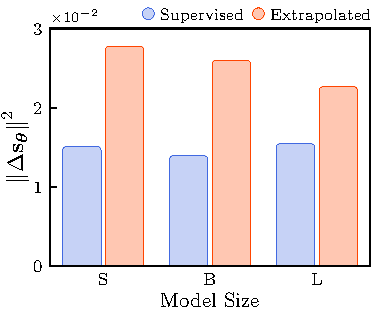
\includegraphics[width=0.9\textwidth]{figures/performance/repa_motivation}
    \vskip -0.5\baselineskip
    \caption{\textbf{Effect of REPA on the learned score $\rvs_\rvtheta$.} Greater change $\|\Delta \rvs_\rvtheta\|^2$ occurs for \coloredul{xred}{extrapolated scores} than for \coloredul{xblue}{supervised scores}.} \label{fig:repa_mot}
\end{figure}
\end{minipage}

\iclronly{
\textbf{Motivation.}~Recall that the DSM loss in~\Cref{eq:dsm-rewritten} measures how well a model fits the empirical score in the supervision region, serving as a measurement of \emph{supervision}. This supervision loss typically correlates with generative performance: as model size increases, both supervision loss and FID decrease. However, as seen in the REPA case above--where supervision changes were minor despite large FID improvements--\emph{supervision loss alone cannot fully explain FID}. This motivates us to decompose the generative performance into two components: supervision and extrapolation.
}

\neuripsonly{\vspace{-0.5\baselineskip}}
\subsection{Decomposed Analysis of Generative Performance}  \label{sec:scaling-analysis}
We introduce our framework for analyzing generative performance, which can be formulated as
{
\neuripsonly{
\setlength{\abovedisplayskip}{4pt}
\setlength{\belowdisplayskip}{4pt}
}
\begin{equation} \label{eq:decomp}
    \text{Generative Performance} := \text{FID} = \xsienna{f_{\text{extrapolation}}}(\xxgreen{\text{supervision loss } \Ls}).
\end{equation}
}%
In words, generative performance is decomposed into two components: \xxgreen{(i) supervision loss $\Ls$}, which measures how well the empirical score is fitted by the \emph{model}, and \xsienna{(ii) extrapolation function $f_\text{extrapolation}$}, which characterizes the extrapolation behavior of the \emph{training recipe}. Conceptually, ${f_{\text{extrapolation}}}$ acts as a transfer function mapping supervision loss to generative performance. Figure~\ref{fig:pat-verification-a} illustrates this: for a fixed training recipe A, represented by ${f^\text{A}_{\text{extrapolation}}}$, smaller supervision loss leads to better FID (\xsienna{\emph{solid line}}). Changing the training recipe to B, e.g., modifying the architecture or adding a regularization term, alters the extrapolation function to ${f^\text{B}_{\text{extrapolation}}}$ (\xsienna{\emph{dashed lines}}).

\newenvironment{tmpfigure2}
  {\venueifelse{\begin{figure}[t]}{\begin{figure}[b]}}
  {\end{figure}}

\begin{tmpfigure2}
    \neuripsonly{\vspace{-1.5\baselineskip}}
    \centering
    \begin{subfigure}[t]{0.325\textwidth}
        \centering
        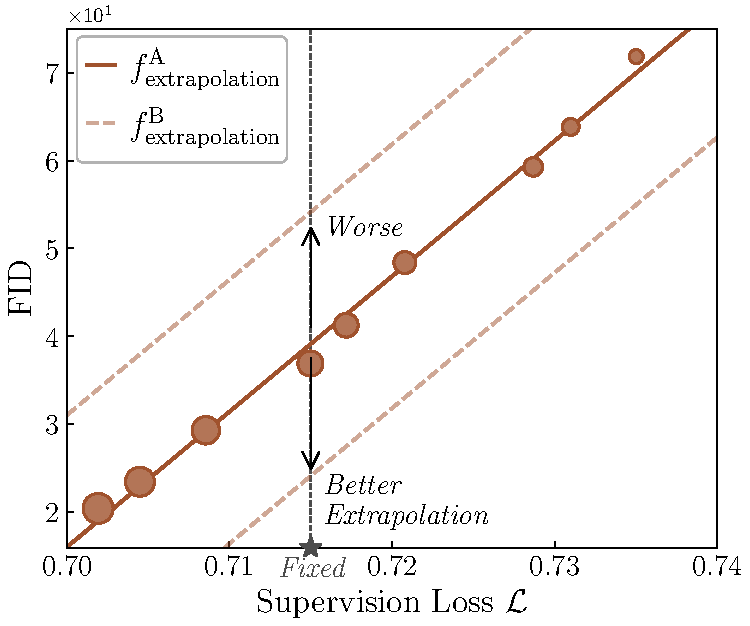
\includegraphics[height=0.86\textwidth]{figures/performance/pat_verification_a}
        % \vskip -0.3\baselineskip
        % \caption{
        % \xsienna{\textbf{Scaling law}}
        % % Supervision loss vs.\ FID, enabling disentanglement of extrapolation from supervision.
        % }
        \phantomcaption
        \label{fig:pat-verification-a}
    \end{subfigure}
    \hfill
    \begin{subfigure}[t]{0.325\textwidth}
        \centering
        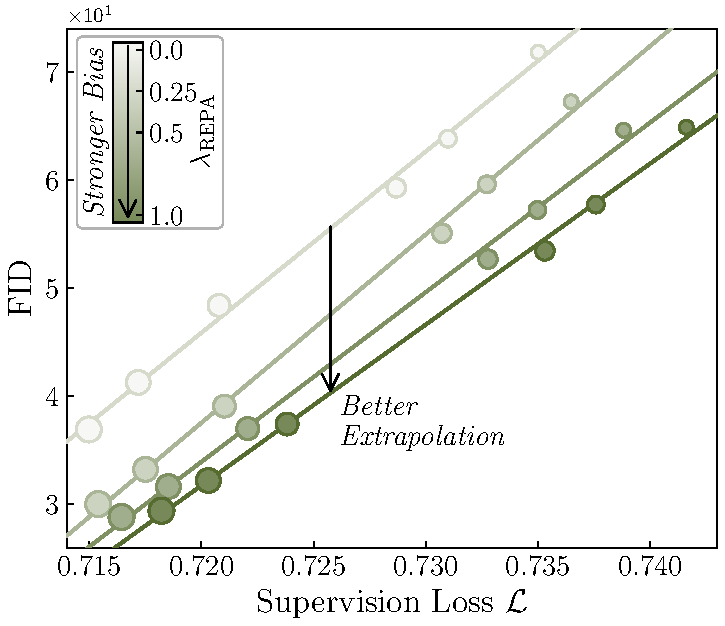
\includegraphics[height=0.86\textwidth]{figures/performance/pat_verification_c}
        % \vskip -0.3\baselineskip
        % \caption{
        % \xolive{\textbf{REPA}}
        % % Varying Alignment strengths $\lamrepa=\{0.0, 0.25, 0.5, 1.0\}$.
        % }
        \phantomcaption
        \label{fig:pat-verification-b}
    \end{subfigure}
    \hfill
    \begin{subfigure}[t]{0.325\textwidth}
        \centering
        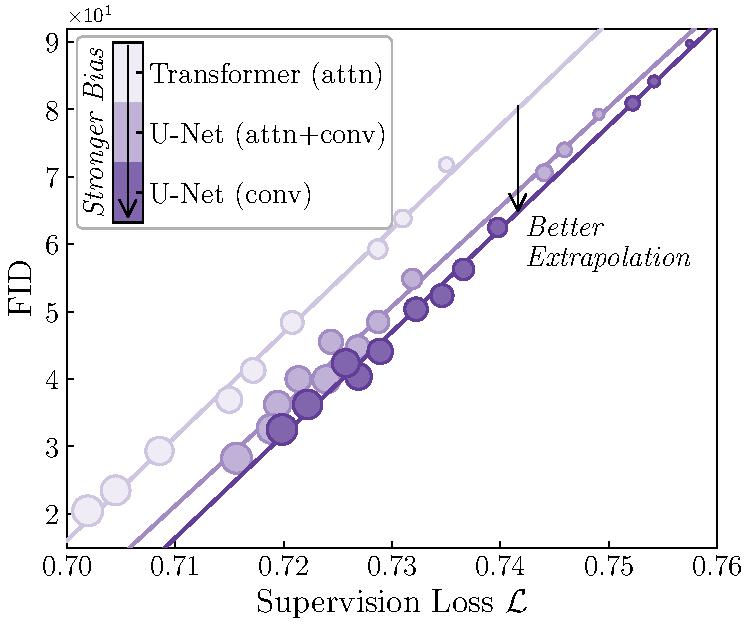
\includegraphics[height=0.86\textwidth]{figures/performance/pat_verification_b}
        % \vskip -0.3\baselineskip
        % \caption{
        % \xxpurple{\textbf{Transformer vs.\ U-Net}}
        % % From Transformer (attn) $\to$ U-Net (attn+conv) $\to$ U-Net (conv).
        % }
        \phantomcaption
        \label{fig:pat-verification-c}
    \end{subfigure}
    \vskip -1.5\baselineskip
    \caption{
    \textbf{Illustration of the decomposed analysis of generative performance.} (a) FID (\emph{$y$-axis}) is plotted as a linear function $f_\text{extrapolation}$ (\xsienna{\emph{line}}) of supervision loss $\Ls$ (\emph{$x$-axis}). $f_\text{extrapolation}$ depends on the training recipe (A vs.\ B) and is more efficient when shifted downward. Our analysis shows that (b) \xolive{REPA} and (c) \xxpurple{U-Net (vs.\ transformers)} yield more efficient $f_\text{extrapolation}$, i.e., \emph{better extrapolation behavior}. Marker size indicates each model’s total training compute (FLOPs).
    }
    \label{fig:pat-verification}
    \vskip -1.75\baselineskip
\end{tmpfigure2}

This framework provides a principled way to assess the efficiency of a \emph{training recipe alone}. A downward shift of the ${f_{\text{extrapolation}}}$ line indicates greater efficiency--achieving better FID under the same supervision loss--while an upward shift signals reduced efficiency in converting supervision into generative performance. As shown in \Cref{fig:pat-verification-b}, consistent with our earlier observations, REPA yields a notably efficient ${f_{\text{extrapolation}}}$ for diffusion models, explaining much of its empirical success.


\textbf{Transformer vs.\ U-Net.}~We next examine the impact of architecture--an important axis of the training recipe--by comparing transformer (attention), U-Net (convolution), and U-Net (attention+convolution) models. As shown in \Cref{fig:pat-verification-c}, (i) architectures with more convolutional layers exhibit more efficient extrapolation behavio (downward line shift); but (ii) for a fixed compute budget (marker size), convolution-based architectures have much worse supervision loss than attention-based counterparts. In summary, transformers, compared to U-Nets, yield worse extrapolation efficiency ($\Ls \to \text{FID}$), but much scalable supervision efficiency ($\text{FLOPs} \to \Ls$). This decomposition explains the trend toward transformers for large-scale diffusion training: taking the chain of the two factors, transformers achieve better overall compute efficiency ($\text{FLOPs} \to \text{FID}$). Our results also suggest that one could combine the best of both worlds--the extrapolation efficiency of U-Nets and the supervision efficiency of transformers--as in recent works~\citep{tian2024u,wang2024flowdcn}.
\vspace{-0.22in}
\subsection{Unified Hypothesis for Better Generative Performance} \label{sec:pat}
\vspace{-0.02in}
In \Cref{sec:scaling-analysis}, we introduced a framework for quantifying the extrapolation behavior of different training recipes and presented examples that yield more efficient $\xsienna{f_{\text{extrapolation}}}$, potentially leading to improved generative performance—a property of practical interest. This naturally raises the question: \emph{is there a simple principle for designing training recipes that induce more efficient extrapolation?} To this end, we propose a unified hypothesis: \emph{\xxgreen{Perception-Aligned Training}} (PAT).


\newcommand{\tg}[1]{%
  \tikz[baseline=0.06ex]\draw[fill=#1, draw=black, line width=0.75pt] (0,0) -- (0.2,0) -- (0.1,0.2) -- cycle;\xspace
}
\newcommand{\sq}[1]{%
  \tikz[baseline=0.06ex]\draw[fill=#1, draw=black, line width=0.75pt] (0,0) -- (0.2,0) -- (0.2,0.2) -- (0,0.2) -- cycle;\xspace
}
\newcommand{\tdA}{\tg{xblue}}
\newcommand{\tdB}{\tg{xcyan}}
\newcommand{\tdC}{\sq{xcyan}}
\newcommand{\tdD}{\sq{xlightcyan}}
\newcommand{\ellipseicon}[1]{%
  \tikz[baseline=-0.55ex]\shade[shading=radial, inner color=#1!100, outer color=#1!0, draw=none]
      (0,0) ellipse [x radius=0.35cm, y radius=0.15cm];\xspace
}

\begin{wrapfigure}{r}{0.45\textwidth}
    \centering
    \vskip -1.5\baselineskip
    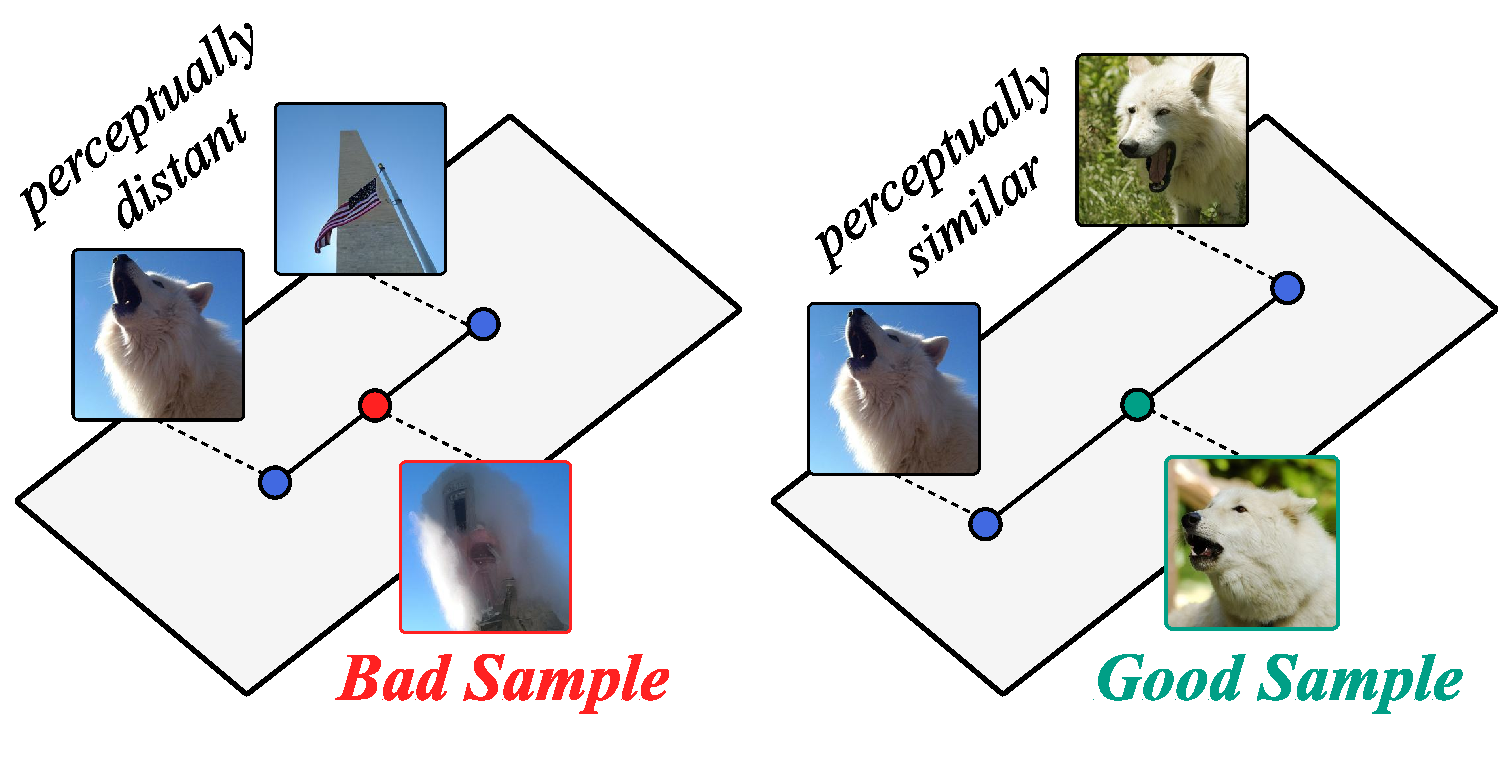
\includegraphics[width=0.45\textwidth]{figures/performance/good_generation}
    \vskip -\baselineskip
    \caption{\textbf{\xxgreen{Good} vs.\ \xred{bad} samples and their connection to \emph{perception}.}}
    \label{fig:good-generation}
    \vskip -2\baselineskip
\end{wrapfigure}
\textbf{PAT.} As shown in \Cref{sec:extrapolation}, a diffusion model \emph{extrapolates} beyond the supervision region to generate samples; this geometrically corresponds to \emph{interpolating} among training images. \Cref{fig:good-generation} shows two scenarios: perceptually distant images may be close in Euclidean space, so naive interpolation produces perceptually \xred{bad samples}; when the space is aligned with \emph{perception}, it yields perceptually \xxgreen{good samples}. This highlights the importance of perception and motivates the following hypothesis:


\begin{claim} \label{claim:good-extrapolation}
Aligning a neural network with perception leads to better extrapolation behavior.
\end{claim}

\iclronly{
The principle of PAT is illustrated in \Cref{fig:pat-def}. Formally, PAT refers to any training recipe that encourages a neural network $\rvs_\rvtheta$ to produce closely aligned outputs $\rvs_\rvtheta (\rvz_t, t)$ for perceptually close inputs $\rvz_t$. Below, we present three representative instances of PAT, demonstrating how it unifies many practical training approaches (see \Cref{app:pat-examples} for further details). We also verify our hypothesis for each instance using 2D toy data (\Cref{app:pat-toy}).
}
\neuripsonly{
The principle of PAT is illustrated in \Cref{fig:pat-def}. Formally, PAT refers to any training recipe that encourages a neural network $\rvs_\rvtheta$ to produce closely aligned outputs $\rvs_\rvtheta (\rvz_t, t)$ for perceptually close inputs $\rvz_t$. We present three representative instances of PAT in \Cref{fig:pat-space,fig:pat-representation,fig:pat-architecture}, which together unify a wide range of practical training approaches, including \xblue{equivariant or perceptually aligned VAEs~\citep{kouzelis2025eq,yao2025reconstruction}}, \xolive{representation-learning-based methods~\citep{yu2024representation,gao2023masked}}, and \xxpurple{recent architectural advances~\citep{tian2024u,wang2024flowdcn}}, as detailed in \Cref{app:pat-examples}. We also verify our PAT hypothesis using 2D toy data in \Cref{app:pat-toy}.
}


\begin{tmpfigure2}
    \neuripsonly{\vskip -0.5\baselineskip}
    \vskip -0.5\baselineskip
    \centering
    \begin{subfigure}[t]{0.48\textwidth}
        \centering
        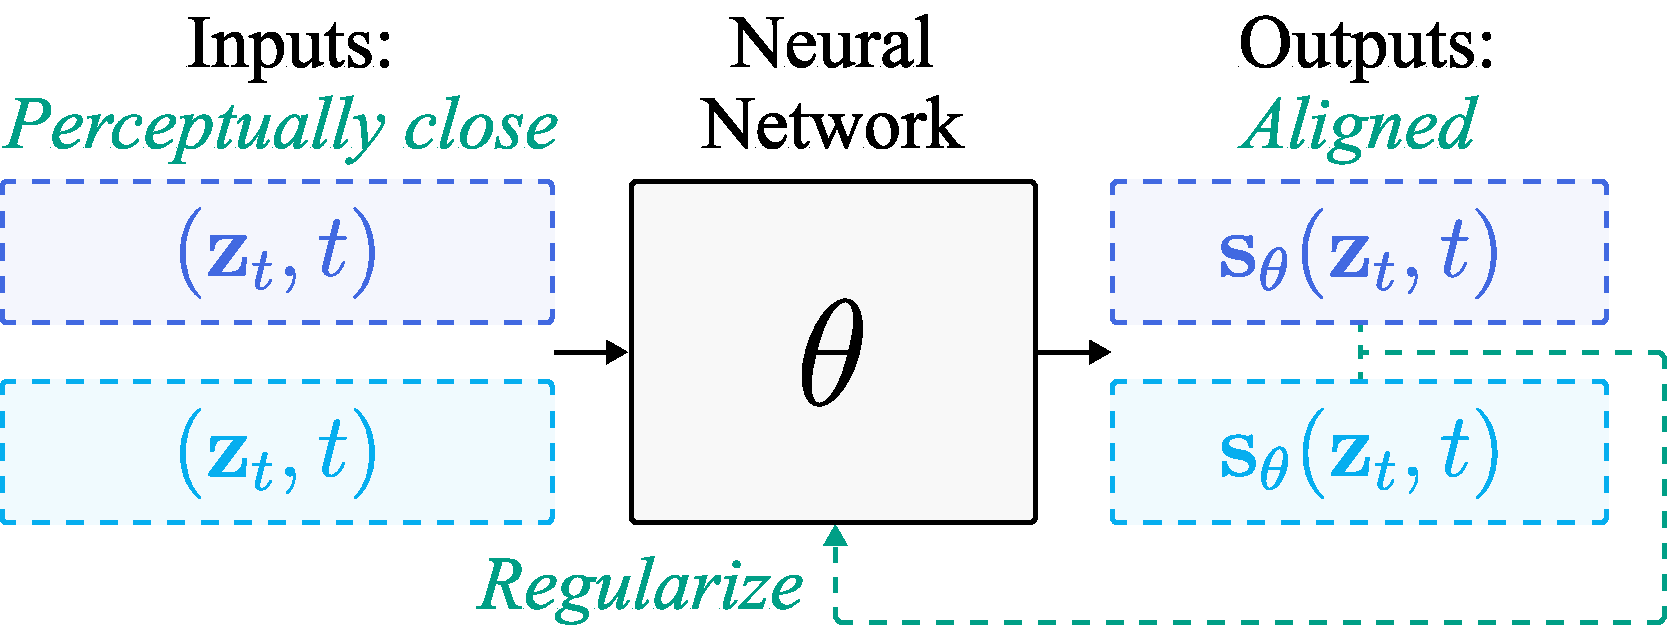
\includegraphics[width=\textwidth]{figures/performance/pat_def}
        \caption{\textbf{Definition of \xxgreen{PAT.}}}
        \label{fig:pat-def}
    \end{subfigure}
    \hfill
    \begin{subfigure}[t]{0.48\textwidth}
        \centering
        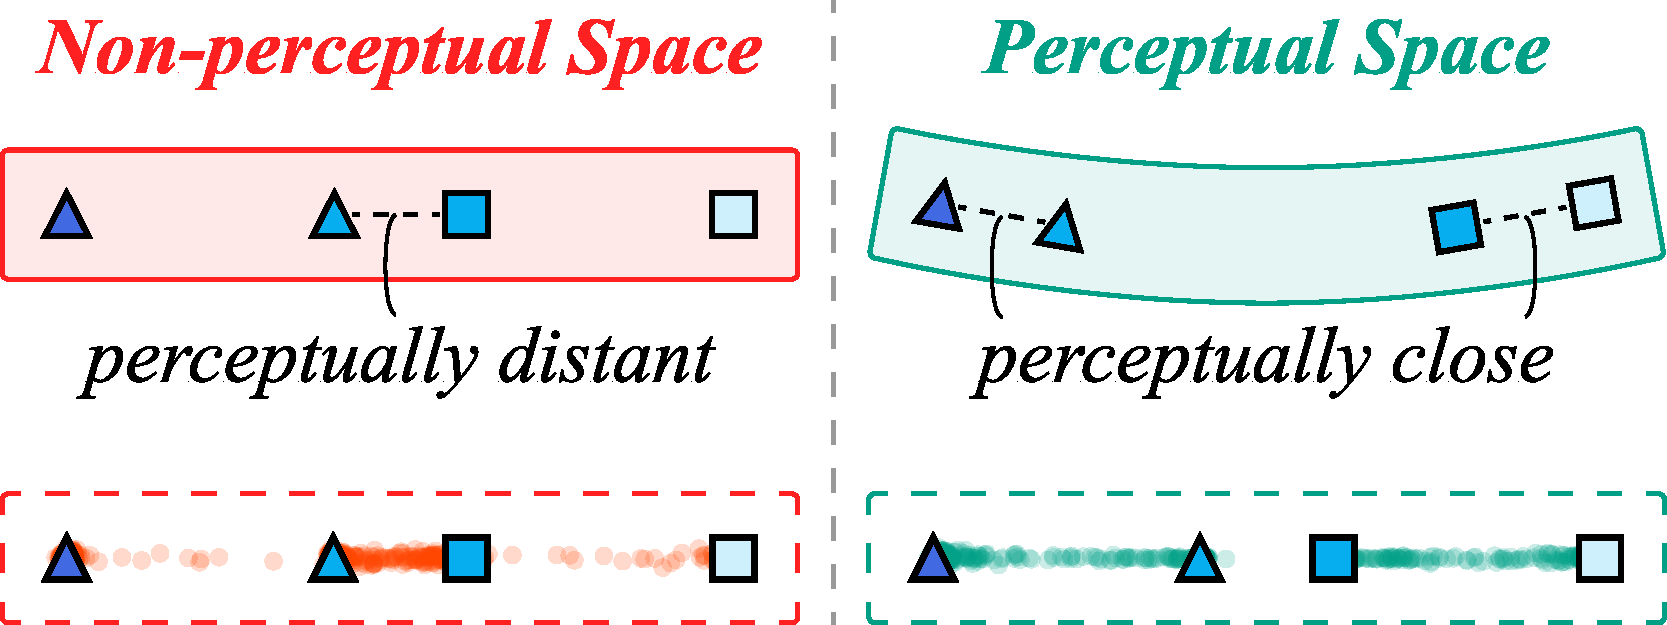
\includegraphics[width=\textwidth]{figures/performance/pat_space}
        \caption{\xblue{\textbf{Aligning diffusion space.}}}
        \label{fig:pat-space}
    \end{subfigure}
    \vskip 0.2\baselineskip
    \begin{subfigure}[t]{0.48\textwidth}
        \centering
        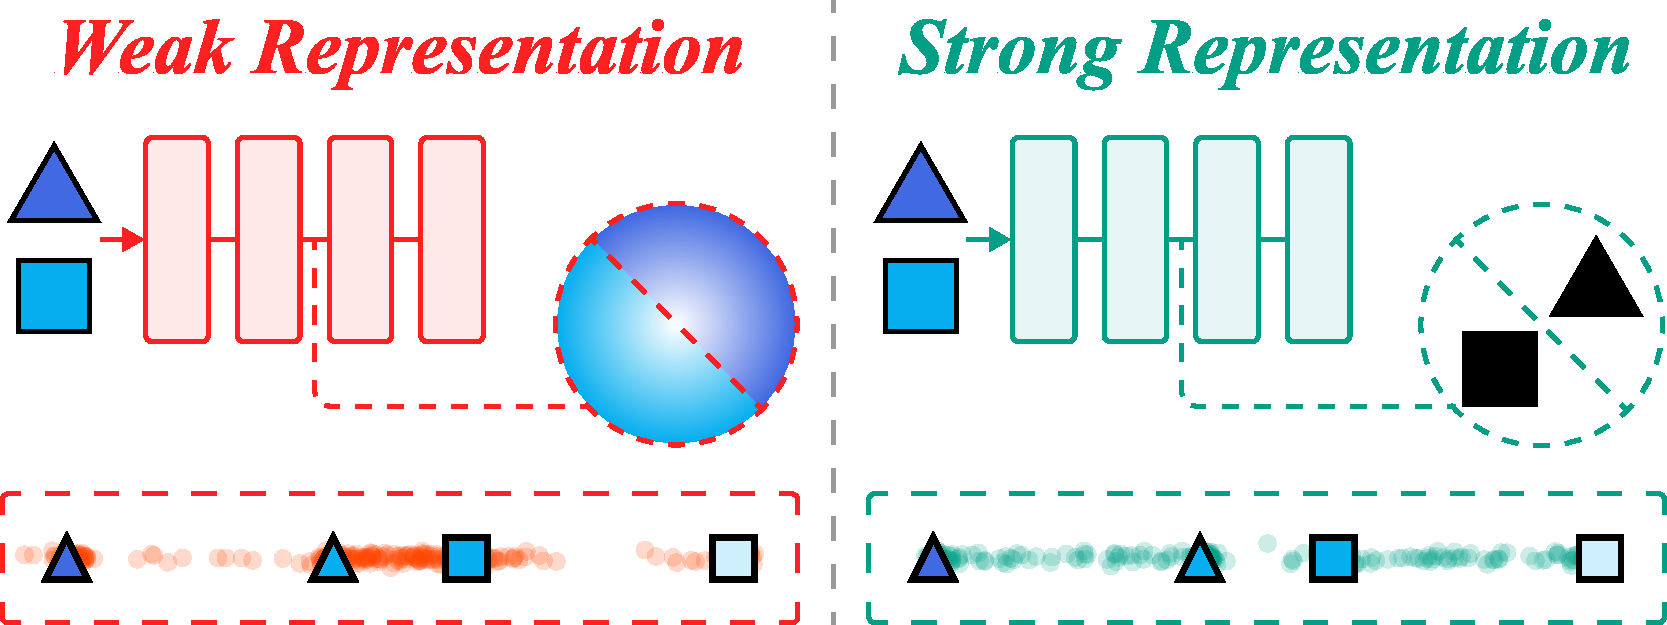
\includegraphics[width=\textwidth]{figures/performance/pat_representation}
        \caption{\xolive{\textbf{Aligning representation.}}}
        \label{fig:pat-representation}
    \end{subfigure}
    \hfill
    \begin{subfigure}[t]{0.48\textwidth}
        \centering
        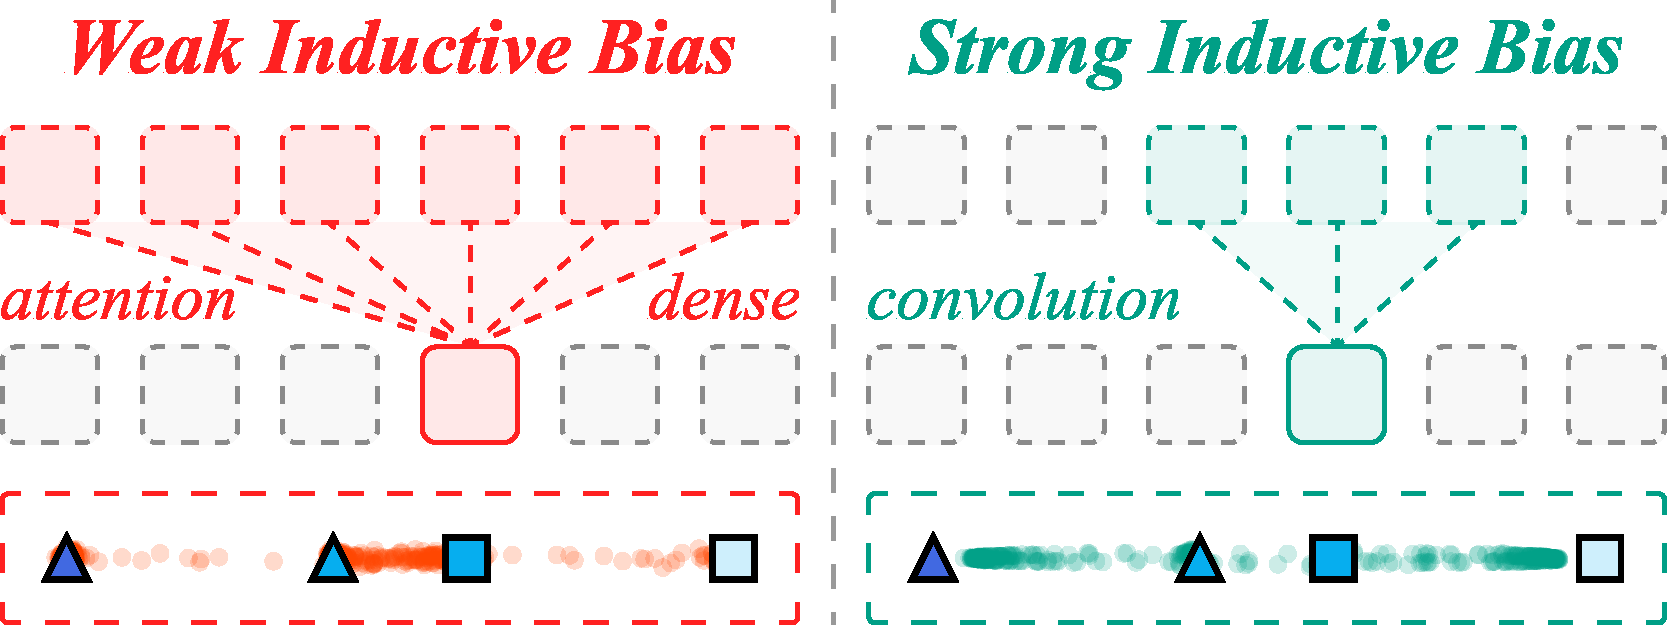
\includegraphics[width=\textwidth]{figures/performance/pat_architecture}
        \caption{\xxpurple{\textbf{Aligning architectural bias.}}}
        \label{fig:pat-architecture}
    \end{subfigure}
    \venueifelse{\vskip -0.5\baselineskip}{\vskip -0.25\baselineskip}
    \caption{\textbf{Illustration of \xxgreen{\emph{Perception-Aligned Training} (PAT)} with toy experiment results.}
    \xxgreen{PAT regularizes} a neural network $\theta$ to output \xxgreen{\emph{aligned}} scores $\rvs_\theta$ for \xxgreen{\emph{perceptually close}} inputs $\rvz_t$. Many successful training techniques can be unified under this view, categorized as the three instances.} \label{fig:pat}
    % For each: \emph{Top}, visual explanations; \emph{Bottom}, experiment results; \textbf{\emph{Left}, \coloreddashul{xred}{without PAT}; \emph{Right}, \coloreddashul{xxgreen}{with PAT}.}}
    \vskip -\baselineskip
\end{tmpfigure2}


\iclronly{
\textbf{\xblue{Aligning Diffusion Space.}}~The most straightforward instance of PAT is training a model in a perceptually aligned space (\Cref{fig:pat-space}). Pixel space and standard VAE latent space, on which diffusion models are commonly trained, often entangle non-perceptual factors~\citep{skorokhodov2025improving}, making Euclidean distance a poor proxy for perceptual similarity. In contrast, a perceptually aligned space allows a smooth score network $\rvs_\rvtheta$ to naturally produce consistent outputs for perceptually similar inputs. This perspective explains the success of methods that construct perceptually meaningful latent spaces, such as EQ-VAE~\citep{kouzelis2025eq} and VA-VAE~\citep{yao2025reconstruction}.

\textbf{\xolive{Aligning Representation.}}~Another approach aligns the model’s internal representation with perception (\Cref{fig:pat-representation}). While keeping output supervision unchanged, the training objective encourages perceptually meaningful intermediate features, which implicitly regularize the outputs. Empirically, this yields more favorable extrapolation (\Cref{fig:pat-verification-b}). Methods incorporating representation learning into diffusion training--REPA~\citep{yu2024representation} and MaskDiT~\citep{zheng2023fast}--are examples.

\textbf{\xxpurple{Aligning Architectural Bias.}}~A third instance is aligning the network's inductive bias with perception (\Cref{fig:pat-architecture}). For images, convolution imparts translational equivariance and locality, aligning well with perceptual invariance such as translation or cropping. This explains the reason why convolution-based architectures tend to induce a more efficient extrapolation function $f_{\text{extrapolation}}$ (\Cref{fig:pat-verification-c}). However, as noted in \Cref{sec:scaling-analysis}, these designs are less favorable in supervision efficiency ($\text{FLOPs} \to \Ls$), which often limits their practical effectiveness at large training scales.
}


\textbf{Discussion.} We posit that a diffusion model's training efficiency decomposes into \textbf{(i)} \emph{supervision efficiency}: how well the model fits the training data, and \textbf{(ii)} \emph{extrapolation efficiency}: how this fit translates into generation performance. This decomposition enables a thorough analysis of different \emph{training recipes}, beyond simply comparing per-model FID. With this perspective, \xxgreen{PAT} offers a unified principle for designing training methods that induce a favorable extrapolation function, i.e., improving \textbf{(ii)}. However, PAT can sometimes weaken \textbf{(i)}; thus, maximizing generative performance under a fixed compute requires balancing supervision and extrapolation. Finally, we emphasize that \textbf{\xsienna{these practical tools are a natural byproduct of \ours}, \xxpurple{impossible with \common}}.

\vspace{-0.5\baselineskip}
